\begin{frame}
\frametitle{Как выглядит физическая память?}

\only<1>{
\begin{figure}
  \centering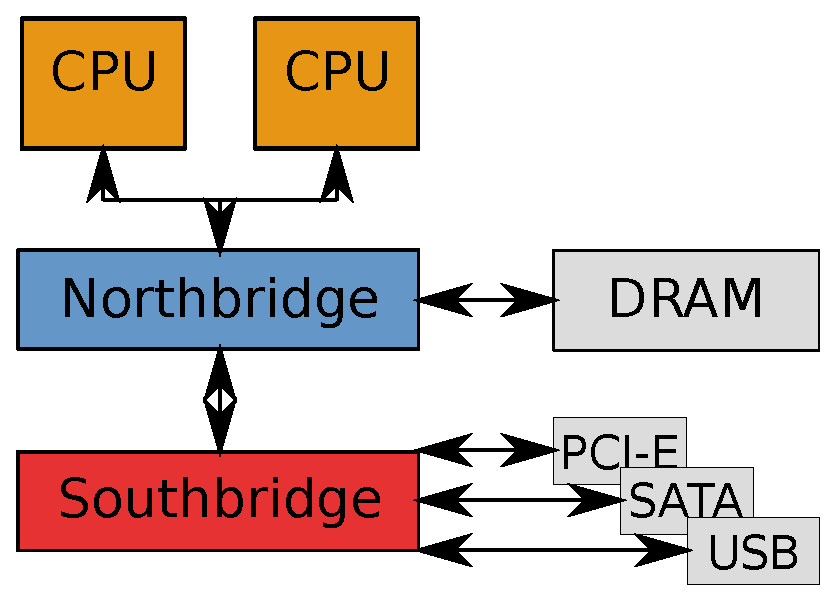
\includegraphics[width=.8\linewidth]{arch-uma}
  \caption{Classical UMA Architecture}
\end{figure}}
\only<2>{
\begin{figure}
  \centering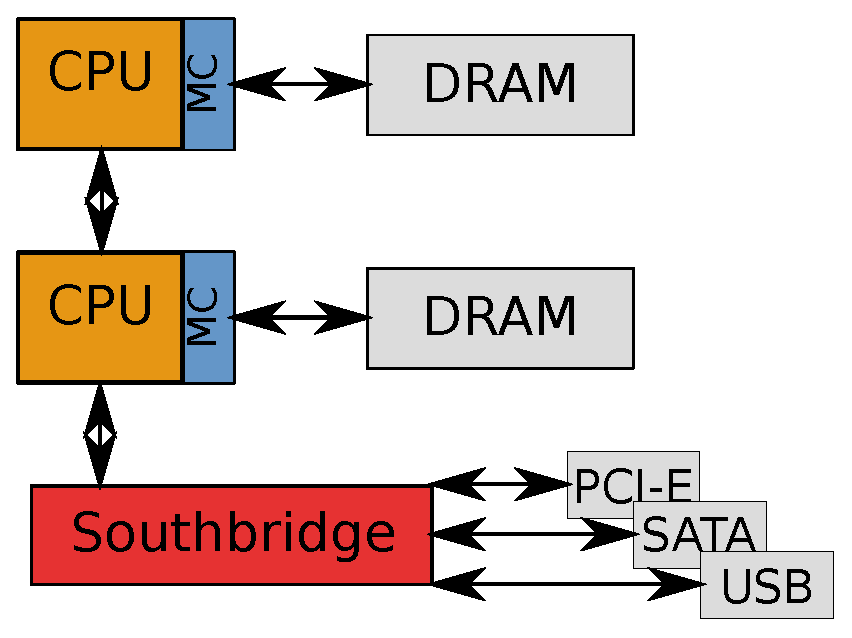
\includegraphics[width=.8\linewidth]{arch-numa}
  \caption{NUMA Architecture}
\end{figure}}

\end{frame}

\begin{frame}
\frametitle{Как выглядит физическая память?}

\onslide<1->{
Память не однородна:

\begin{itemize}
  \item адреса могут вообще быть не доступны - память не отображена никуда;
  \item адреса могут быть отображены на устройства - особые правила доступа/кеширования;
  \item разные адреса могут иметь разное время доступа с разных CPU (NUMA);
\end{itemize}}

\onslide<2->{Нужна карта памяти!}

\end{frame}

\begin{frame}
\frametitle{Где взять карту памяти?}

\begin{itemize}
  \item<1-> из документации чипсета
  \item<2-> из device tree
    \begin{itemize}
      \item кто-то все равно должен взять документацию чипсета и описать память в нужном формате и передать загрузчику
    \end{itemize}
  \item<3-> BIOS/UEFI или их аналог
    \begin{itemize}
      \item BIOS int \$0x15, функции 0xe820 или 0xe801
      \item UEFI GetMemoryMap
    \end{itemize}
  \item<4-> спросить у загрузчика (где ее берет загрузчик - не наше дело)
\end{itemize}
\end{frame}

\begin{frame}
\frametitle{Типичная карта памяти}

Такие регионы памяти, например, может сообщать QEMU через multiboot загрузчик:

\begin{itemize}
  \item \texttt{0x00000000-0x0009fbff, Available}
  \item \texttt{0x0009fc00-0x0009ffff, Reserved}
  \item \texttt{0x000f0000-0x000fffff, Reserved}
  \item \texttt{0x00100000-0x07ffdfff, Available}
  \item \texttt{0x07ffe000-0x07ffffff, Reserved}
  \item \texttt{0xfffc0000-0xffffffff, Reserved}
\end{itemize}

\end{frame}
